\documentclass[10pt]{beamer}

\usepackage{tikz}
\usepackage{tikz-cd}

\newtheorem{conjecture}{Conjecture}
\newtheorem{exercise}{Exercise}

\setbeamertemplate{footline}[page number]

\title{Algebraising foundations of elliptic curves}

\author{David Kurniadi Angdinata \\ (joint work with Junyan Xu)}

\institute{London School of Geometry and Number Theory}

\date{Thursday, 13 February 2025}

\begin{document}

\frame{\titlepage}

\begin{frame}[t]{Introduction}

\emph{Elliptic curves} are algebraic curves given by cubic equations.

\begin{center}
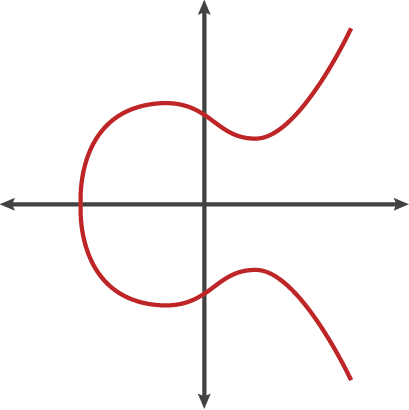
\includegraphics[width=0.5\textwidth]{ellipticcurve.png}
\end{center}

Their set of points can be endowed with a \emph{group law}.

\end{frame}

\begin{frame}[t]{Motivation}

Why should we care about elliptic curves?

\pause

\vspace{0.5cm} They are prevalent in modern number theory.
\begin{itemize}
\item Wiles proved \emph{Fermat's last theorem} by drawing a correspondence between certain elliptic curves and certain \emph{modular forms}.
\item The \emph{Birch and Swinnerton-Dyer conjecture} predicts the arithmetic behaviour of elliptic curves based on their \emph{L-functions}.
\end{itemize}

\pause

\vspace{0.5cm} They see many computational applications.
\begin{itemize}
\item Intractability of the \emph{discrete logarithm problem} for elliptic curves forms the basis behind many public key cryptographic protocols.
\item The \emph{Atkin--Morain primality test} and \emph{Lenstra's factorisation method} use elliptic curves and are two of the fastest known algorithms.
\end{itemize}

\vspace{0.5cm} Formalising the theory of elliptic curves would be great!

\end{frame}

\begin{frame}[t]{History}

There is much previous work in various interactive theorem provers.

\begin{itemize}
\item Anthony Fox, Mike Gordon, and Joe Hurd (2006) formalised a definition of an elliptic curve in HOL4 over an arbitrary field $ F $.

\pause

\item Laurent Th\'ery (2007) formalised a \emph{direct} proof of the group law on an elliptic curve in Coq, assuming $ \mathrm{char}(F) \ne 2, 3 $.

\pause

\item Evmorfia-Iro Bartzia and Pierre-Yves Strub (2014) formalised a \emph{conceptual} proof of the group law in Coq, assuming $ \mathrm{char}(F) \ne 2, 3 $.

\pause

\item Thomas Hales and Rodrigo Raya (2020) formalised a \emph{direct} proof of the group law in Isabelle, assuming $ \mathrm{char}(F) \ne 2 $.

\pause

\item Junyan Xu and I (2023) formalised a \emph{novel conceptual} proof of the group law in Lean, \emph{with no assumptions on $ \mathrm{char}(F) $}.

\pause

\item Junyan Xu and I (2024) discovered gaps in the standard proof of the \emph{multiplication-by-$ n $ formula} on an elliptic curve, filled them in with \emph{novel} arguments, and formalised the entire proof in Lean.
\end{itemize}

\end{frame}

\begin{frame}[t]{Elliptic curves}

An \textbf{elliptic curve} over a field $ F $ is a smooth projective curve $ E $ over $ F $ of genus one, equipped with a distinguished point $ \mathcal{O} $ defined over $ F $.

\vspace{0.5cm} These are all notions from modern algebraic geometry.
\begin{itemize}
\item A \textbf{curve} is a variety \footnote{integral separated scheme of finite type over $ \mathrm{Spec}(F) $} of dimension one as a topological space.
\item \textbf{Projective} means there is a closed immersion $ E \hookrightarrow \mathrm{Proj}(F[X_i]) $.
\item \textbf{Smooth} essentially means all $ \mathcal{O}_{E, \overline{x}} $ are regular local rings.
\item \textbf{Genus} is the dimension of $ H^1(E, \mathcal{O}_E) $ as an $ F $-vector space.
\end{itemize}

\pause

\vspace{0.5cm} In \texttt{mathlib}, we have schemes (Aug 2020), integral schemes (Dec 2021), projective schemes (Apr 2022), finite type morphisms (Oct 2022), Krull dimensions (May 2023), separated morphisms (Jun 2024), smooth morphisms (Jul 2024), and sheaf cohomology (Jul 2024).

\pause

\vspace{0.5cm} Thanks to the work of Andrew Yang, Christian Merten, Jo\"el Riou, and others, we can \emph{almost} formalise the definition of elliptic curves in Lean!

\end{frame}

\begin{frame}[t]{Elliptic curves in \texttt{mathlib}}

\begin{corollary}[of the Riemann--Roch theorem]
The set of points of an elliptic curve over $ F $ is the vanishing locus of
$$ \mathcal{E} := Y^2 + a_1XY + a_3Y - (X^3 + a_2X^2 + a_4X + a_6), $$
for some $ a_i \in F $ such that $ \Delta \ne 0 $, \footnote{\tiny $ \Delta := -(a_1^2 + 4a_2)^2(a_1^2a_6 + 4a_2a_6 - a_1a_3a_4 + a_2a_3^2 - a_4^2) - 8(2a_4 + a_1a_3)^3 - 27(a_3^2 + 4a_6)^2 + 9(a_1^2 + 4a_2)(2a_4 + a_1a_3)(a_3^2 + 4a_6) $} with an extra point at infinity $ \mathcal{O} $.
\end{corollary}

\pause

\vspace{0.5cm} In other words, there is an equivalence of categories
$$ \{\text{elliptic curves over} \ F\} \cong \{(a_1, a_2, a_3, a_4, a_6) \in F^5 \ \text{such that} \ \Delta \ne 0\}. $$

\pause

In \texttt{mathlib}, an \textbf{elliptic curve} $ E $ over a ring $ R $ is the data of tuples $ (a_1, a_2, a_3, a_4, a_6) \in R^5 $ and a proof that $ \Delta \in R^\times $. A \textbf{point} on $ E $ is then a sum type of $ \mathcal{O} $ and \textbf{affine points} $ (x, y) \in R^2 $ such that $ \mathcal{E}(x, y) = 0 $.

\pause

\vspace{0.5cm} The arithmetic can be formalised independently of the algebraic geometry.

\end{frame}

\begin{frame}[t]{The group law}

The set of points $ E(F) $ can be endowed with a geometric addition law.

\begin{center}
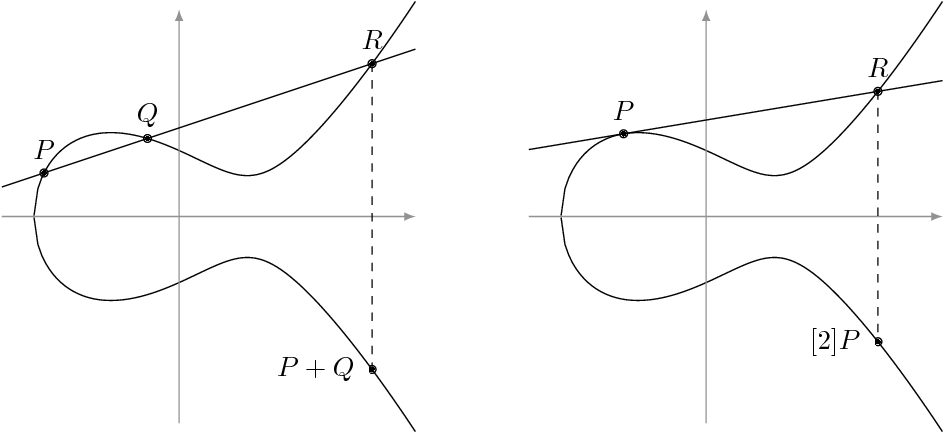
\includegraphics[width=\textwidth]{grouplaw.png}
\end{center}

\pause

\begin{theorem}[the group law]
This addition law makes $ E(F) $ an abelian group with identity $ \mathcal{O} $.
\end{theorem}

\end{frame}

\begin{frame}[t]{The group law in \texttt{mathlib}}

In \texttt{mathlib}, the addition law is given by explicit rational functions.

\vspace{0.5cm} For instance, $ (x_1, y_1) + (x_2, y_2) := (x_3, y_3) $, where
\begin{align*}
x_3 & := \lambda^2 + a_1\lambda - a_2 - x_1 - x_2, \\
y_3 & := -\lambda(x_3 - x_1) - y_1 - a_1x_3 - a_3.
\end{align*}

\pause

Here, the slope $ \lambda $ is given by
$$ \lambda := \begin{cases} \dfrac{y_1 - y_2}{x_1 - x_2} & x_1 \ne x_2 \vspace{0.2cm} \\ \dfrac{3x_1^2 + 2a_2x_1 + a_4 - a_1y_1}{2y_1 + a_1x + a_3} & y_1 \ne -y_1 - a_1x - a_3 \\ \infty & \text{otherwise} \end{cases}. $$

\pause

All of the axioms for an abelian group are easy \emph{except for associativity}.

\end{frame}

\begin{frame}[t]{Associativity}

Associativity is the statement that, for all $ P, Q, R \in E(F) $,
$$ (P + Q) + R = P + (Q + R). $$
In the generic case, \footnote{$ P $, $ Q $, $ R $, $ P + Q $, $ P + R $, and $ Q + R $ are not $ \mathcal{O} $ and have distinct $ X $-coordinates} checking that their $ X $-coordinates are equal is an equality of multivariate polynomials with 26,082 terms!

\pause

\vspace{0.5cm} When $ \mathrm{char}(F) \ne 2, 3 $, a linear change of variables reduces $ \mathcal{E} $ to
$$ \mathcal{E}' := Y^2 - (X^3 + aX + b), $$
for some $ a, b \in F $ such that $ -16(4a^3 + 27b^2) \ne 0 $.

\pause

\vspace{0.5cm} This computation reduces to an equality of polynomials with 2,636 terms.

\pause

\vspace{0.5cm} Automation in an interactive theorem prover enables manipulation of multivariate polynomials with at most 5,000 terms.

\end{frame}

\begin{frame}[t]{A complex uniformisation}

Why should there be a group law in the first place?

\pause

\vspace{0.5cm} Over $ F = \mathbb{C} $, an elliptic curve is just a complex torus $ \mathbb{C} / \Lambda_E $.

\begin{center}
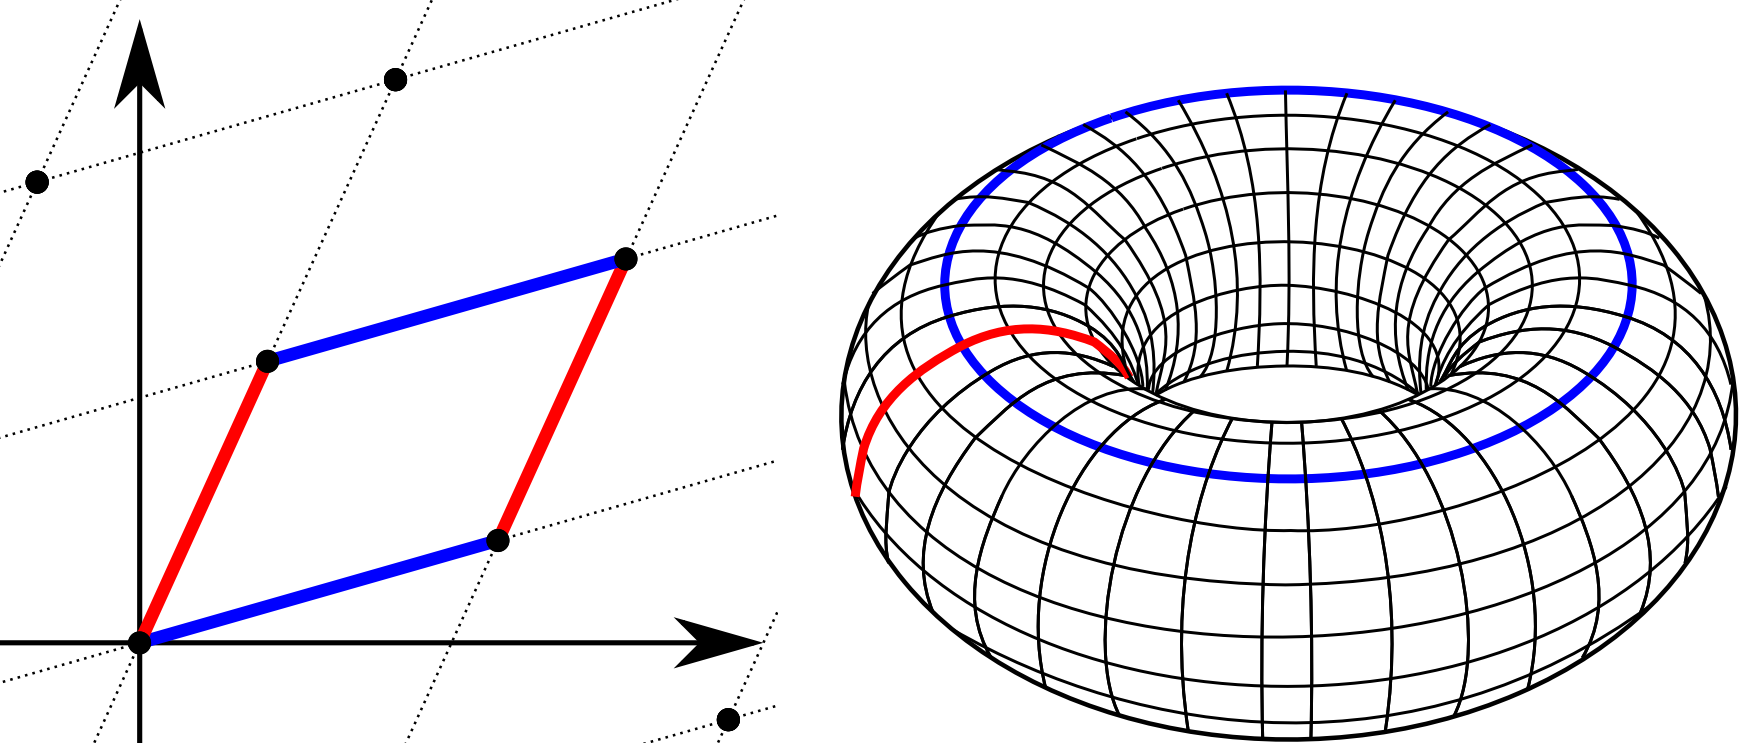
\includegraphics[width=\textwidth]{complextorus.png}
\end{center}

There is an explicit bijection from $ E(\mathbb{C}) $ to $ \mathbb{C} / \Lambda_E $ that preserves the addition law, so the group law on $ \mathbb{C} / \Lambda_E $ can be pulled back to $ E(\mathbb{C}) $.

\end{frame}

\begin{frame}[t]{An algebraic variant}

\only<1-4>{In general, Riemann--Roch gives an explicit bijection from $ E(F) $ to the degree-zero divisor class group $ \mathrm{Pic}_F^0(E) $ that preserves the addition law.}

\only<2-4>{\vspace{0.5cm} While \texttt{mathlib} does not have divisors, it has ideals of integral domains $ D $ and the ideal class group \footnote{group of invertible fractional ideals of $ D $} $ \mathrm{Cl}(D) $, which are \emph{purely commutative algebra}.}

\only<3-4>{\vspace{0.5cm} The map $ E(F) \to \mathrm{Pic}_F^0(E) $ translates to the map
$$
\begin{array}{rcl}
E(F) & \longrightarrow & \mathrm{Cl}(D) \\
\mathcal{O} & \longmapsto & [\langle 1 \rangle] \\
(x, y) & \longmapsto & [\langle X - x, Y - y \rangle]
\end{array},
$$
where $ D $ is the integral domain $ F[X, Y] / \langle\mathcal{E}\rangle $.}

\only<4>{\vspace{0.5cm}
\begin{theorem}[Xu]
Proving that this map is injective only needs linear algebra.
\end{theorem}
}

\end{frame}

\begin{frame}[t]{Multiplication by $ n $}

For each $ n \in \mathbb{Z} $ and each point $ P \in E(F) $, define $ [n](P) := \underbrace{P + \dots + P}_n $.

\pause

\vspace{0.5cm} How many points $ P \in E(\mathbb{C}) $ are there such that $ [n](P) = \mathcal{O} $?

\begin{center}
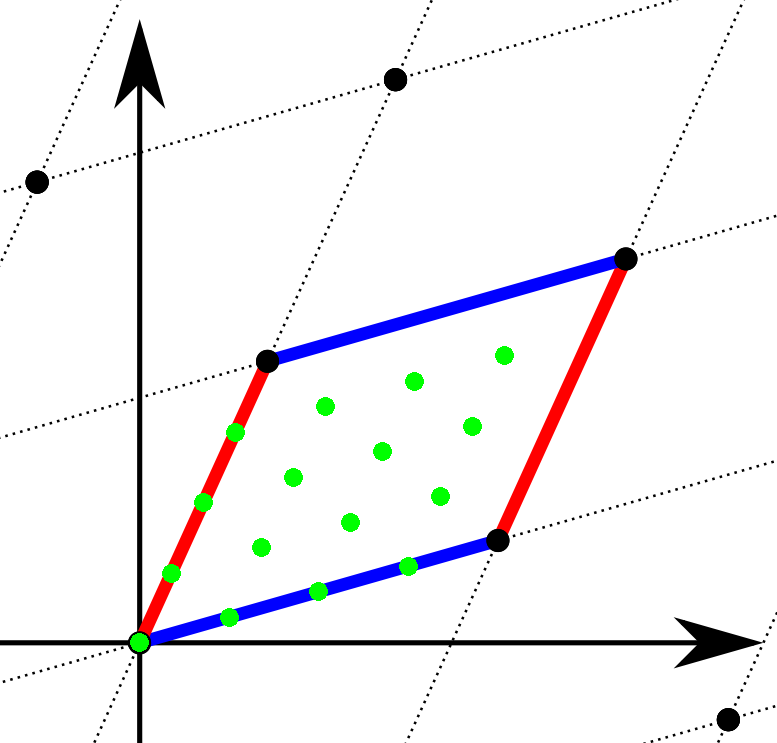
\includegraphics[width=0.5\textwidth]{torsionsubgroup.png}
\end{center}

\end{frame}

\begin{frame}[t]{The $ n $-torsion subgroup}

\only<1-4>{For each $ n \in \mathbb{Z} $, define $ E_F[n] := \{P \in E(F) : [n](P) = \mathcal{O}\} $.

\vspace{0.5cm}
\begin{theorem}[the $ n $-torsion subgroup structure]
If $ \mathrm{char}(F) \nmid n $, then $ E_{\overline{F}}[n] $ is isomorphic to $ (\mathbb{Z} / n)^2 $.
\end{theorem}
}

\only<2-4>{\vspace{0.5cm} When $ \mathrm{char}(F) \ne p $, \visible<3-4>{the \textbf{$ p $-adic Tate module} $ T_pE_{\overline{F}} $ sits in the diagram}
$$
\begin{tikzcd}[ampersand replacement=\&]
{\visible<3-4>{T_pE_{\overline{F}}}} \only<3-4>{\arrow{d}{\sim}} \&[-30] {\visible<3-4>{:= \varprojlim\Big(}}\dots \arrow{r}{[p]} \& E_{\overline{F}}[p^3] \arrow{r}{[p]} \arrow{d}{\sim} \& E_{\overline{F}}[p^2] \arrow{r}{[p]} \arrow{d}{\sim} \& E_{\overline{F}}[p]{\visible<3-4>{\Big)}} \arrow{d}{\sim} \\
{\visible<3-4>{\mathbb{Z}_p^2}} \& {\visible<3-4>{:= \varprojlim\Big(}}\dots \arrow{r}{\bmod p^3} \& (\mathbb{Z} / p^3)^2 \arrow{r}{\bmod p^2} \& (\mathbb{Z} / p^2)^2 \arrow{r}{\bmod p} \& (\mathbb{Z} / p)^2{\visible<3-4>{\Big)}}
\end{tikzcd}.
$$
}

\only<4>{This makes $ T_pE_{\overline{F}} $ a \emph{two-dimensional $ p $-adic Galois representation}. \footnote{crucial in the Mordell--Weil theorem, Tate's isogeny theorem, Serre's open image theorem, Wiles's modularity theorem, the Birch and Swinnerton-Dyer conjecture, etc.}}

\end{frame}

\begin{frame}[t]{An infamous exercise}

\emph{The Arithmetic of Elliptic Curves} by Silverman gives a formula for $ [n](P) $.

\begin{exercise}[3.7(d)]
Let $ n \in \mathbb{Z} $. Prove that for any affine point $ (x, y) \in E(F) $,
$$ [n]((x, y)) = \left(\dfrac{\phi_n(x, y)}{\psi_n(x, y)^2}, \dfrac{\omega_n(x, y)}{\psi_n(x, y)^3}\right). $$
\end{exercise}

\pagebreak

Silverman gives definitions for $ \phi_n, \omega_n \in F[X, Y] $ in terms of certain \emph{division polynomials} $ \psi_n \in F[X, Y] $, which feature in Schoof's algorithm.

\pause

\vspace{0.5cm}

\begin{conjecture}
No one has done Exercise 3.7(d) purely algebraically.
\end{conjecture}

\pause

\vspace{0.5cm} This formula does not account for affine points $ (x, y) \in E(F) $ such that $ \psi_n(x, y) = 0 $, which occurs precisely when $ [n]((x, y)) = \mathcal{O} $.

\end{frame}

\begin{frame}[t]{Projective coordinates}

In projective coordinates, the multiplication-by-$ n $ formula becomes
$$ [n]((x, y)) = [(\phi_n(x, y)\psi_n(x, y), \omega_n(x, y), \psi_n(x, y)^3)]. $$
In \texttt{mathlib}, a \textbf{projective point} is a class of $ (x, y, z) \in F^3 $ such that
$$ y^2z + a_1xyz + a_3yz^2 = x^3 + a_2x^2z + a_4xz^2 + a_6z^3. $$
The point at infinity becomes $ [(0, 1, 0)] $.

\pause

\vspace{0.5cm} More naturally, in projective coordinates with weights $ (2, 3, 1) $,
$$ [n]((x, y)) = [(\phi_n(x, y), \omega_n(x, y), \psi_n(x, y))]. $$
In \texttt{mathlib}, a \textbf{Jacobian point} is a class of $ (x, y, z) \in F^3 $ such that
$$ y^2 + a_1xyz + a_3yz^3 = x^3 + a_2x^2z^2 + a_4xz^4 + a_6z^6. $$
The point at infinity becomes $ [(1, 1, 0)] $.

\end{frame}

\begin{frame}[t]{The polynomials $ \psi_n $}

For any ring $ R $, the \textbf{$ n $-th division polynomial} $ \psi_n \in R[X, Y] $ is given by
\begin{align*}
\psi_0 & := 0, \\
\psi_1 & := 1, \\
\psi_2 & := 2Y + a_1X + a_3, \\
\psi_3 & := {\scriptstyle 3X^4 + (a_1^2 + 4a_2)X^3 + 3(2a_4 + a_1a_3)X^2 + 3(a_3^2 + 4a_6)X + (a_1^2a_6 + 4a_2a_6 - a_1a_3a_4 + a_2a_3^2 - a_4^2)}, \\
\psi_4 & := \psi_2\Bigg(\begin{array}{c} \scriptscriptstyle 2X^6 + (a_1^2 + 4a_2)X^5 + 5(2a_4 + a_1a_3)X^4 + 10(a_3^2 + 4a_6)X^3 + 10(a_1^2a_6 + 4a_2a_6 - a_1a_3a_4 + a_2a_3^2 - a_4^2)X^2 \\ \scriptscriptstyle + ((a_1^2 + 4a_2)(a_1^2a_6 + 4a_2a_6 - a_1a_3a_4 + a_2a_3^2 - a_4^2) - (2a_4 + a_1a_3)(a_3^2 + 4a_6))X \\ \scriptscriptstyle + ((2a_4 + a_1a_3)(a_1^2a_6 + 4a_2a_6 - a_1a_3a_4 + a_2a_3^2 - a_4^2) - (a_3^2 + 4a_6)^2) \end{array}\Bigg), \\
\psi_{2n + 1} & := \psi_{n + 2}\psi_n^3 - \psi_{n - 1}\psi_{n + 1}^3, \\
\psi_{2n} & := \dfrac{\psi_{n - 1}^2\psi_n\psi_{n + 2} - \psi_{n - 2}\psi_n\psi_{n + 1}^2}{\psi_2}, \\
\psi_{-n} & := -\psi_n.
\end{align*}

\pause

In \texttt{mathlib}, $ \psi_n $ is defined in terms of some polynomial $ \Psi_n \in R[X] $ such that $ \psi_n = \Psi_n $ when $ n $ is odd and $ \psi_n = \psi_2\Psi_n $ when $ n $ is even.

\end{frame}

\begin{frame}[t]{The polynomials $ \phi_n $}

The polynomial $ \phi_n \in R[X, Y] $ is given by
$$ \phi_n := X\psi_n^2 - \psi_{n + 1}\psi_{n - 1}. $$

\pause

In \texttt{mathlib}, $ \phi_n $ is defined in terms of some polynomial $ \Phi_n \in R[X] $, since
\begin{align*}
\psi_2^2
& = (2Y + a_1X + a_3)^2 \\
& = 4(Y^2 + a_1XY + a_3Y) + a_1^2X^2 + 2a_1a_3X + a_3^2 \\
& \equiv 4X^3 + b_2X^2 + 2b_4X + b_6 \mod \mathcal{E},
\end{align*}
so $ \psi_n^2 $ and $ \psi_{n + 1}\psi_{n - 1} $ are congruent to polynomials in $ R[X] $.

\pause

\vspace{0.5cm}

\begin{exercise}[3.7(c)]
Let $ n \in \mathbb{Z} $. Prove that $ \phi_n $ and $ \psi_n^2 $ have no common roots.
\end{exercise}

\vspace{0.5cm} This \emph{needs} Exercise 3.7(d) and the assumption that $ \Delta \ne 0 $.

\end{frame}

\begin{frame}[t]{The polynomials $ \omega_n $}

The polynomial $ \omega_n \in R[X, Y] $ is given by
$$ \omega_n := \dfrac{1}{2}\left(\dfrac{\psi_{2n}}{\psi_n} - a_1\phi_n\psi_n - a_3\psi_n^3\right). $$

\pause

\begin{lemma}[Xu]
Let $ n \in \mathbb{Z} $. Then $ \psi_{2n} / \psi_n - a_1\phi_n\psi_n - a_3\psi_n^3 $ is divisible by $ 2 $ in $ \mathbb{Z}[a_i, X, Y] $.
\end{lemma}

\begin{example}[$ a_1 = a_3 = 0 $]
\vspace{-0.5cm}
$$ \omega_2 = \dfrac{\scriptscriptstyle 2X^6 + 4a_2X^5 + 10a_4X^4 + 40a_6X^3 + 10(4a_2a_6 - a_4^2)X^2 + (4a_2(4a_2a_6 - a_4^2) - 8a_4a_6)X + (2a_4(4a_2a_6 - a_4^2) - 16a_6^2)}{2}. $$
\end{example}

\pause

\vspace{0.5cm} Define $ \omega_n $ as the image of the quotient under $ \mathbb{Z}[a_i, X, Y] \to R[X, Y] $.

\vspace{0.5cm} When $ n = 4 $, this quotient has 15,049 terms.

\end{frame}

\begin{frame}[t]{Elliptic divisibility sequences}

Integrality relies on the fact that $ \psi_n $ is an \textbf{elliptic divisibility sequence}.

\begin{exercise}[3.7(g)]
For all $ n, m, r \in \mathbb{Z} $, prove that $ \psi_n \mid \psi_{nm} $ and
$$ \mathrm{ES}(n, m, r) : \psi_{n + m}\psi_{n - m}\psi_r^2 = \psi_{n + r}\psi_{n - r}\psi_m^2 - \psi_{m + r}\psi_{m - r}\psi_n^2. $$
\end{exercise}

Note that $ \mathrm{ES}(n + 1, n, 1) $ gives $ \psi_{2n + 1} $ and $ \mathrm{ES}(n + 1, n - 1, 1) $ gives $ \psi_{2n} $.

\pause

\vspace{0.5cm} Surprisingly, this needs the stronger result that $ \psi_n $ is an \textbf{elliptic net}.

\begin{theorem}[Xu]
Let $ n, m, r, s \in \mathbb{Z} $. Then
\begin{align*}
\mathrm{EN}(n, m, r, s) : \psi_{n + m}\psi_{n - m}\psi_{r + s}\psi_{r - s}
& = \psi_{n + r}\psi_{n - r}\psi_{m + s}\psi_{m - s} \\
& - \psi_{m + r}\psi_{m - r}\psi_{n + s}\psi_{n - s}.
\end{align*}
\end{theorem}

Xu gave an elegant proof of this on Math Stack Exchange.

\end{frame}

\begin{frame}[t]{Ellipticity of $ \psi_n $}

It suffices to prove $ \mathrm{EN}(n, m, r, s) $ by strong induction on $ n $ assuming that $ n, m, r, s \in \mathbb{N} $ \footnote{the complete proof also needs the case when $ n, m, r, s \in \tfrac{1}{2}\mathbb{N} \setminus \mathbb{N} $} such that $ n > m > r > s $. \pause Firstly,
$$ \mathrm{EN}(n, m, 1, 0) = \mathrm{EN}(\tfrac{n + m + 1}{2}, \tfrac{n + m - 1}{2}, \tfrac{n - m + 1}{2}, \tfrac{n - m - 1}{2}). $$
If $ n = m + 1 $, then $ \mathrm{EN}(m + 1, m, 1, 0) $ holds by definition of $ \psi_{2n + 1} $. Otherwise $ n > m + 1 $, then inductive hypothesis applies since $ \tfrac{n + m + 1}{2} < n $. This gives $ \mathrm{EN}(n, m, 1, 0) $ for all $ n, m > 1 $. \pause Furthermore,

\vspace{-0.5cm}
$$
\arraycolsep=0.5pt
\begin{array}{rcrcrcr}
\scriptstyle \mathrm{EN}(n, m, r, 0) & = & \scriptstyle \psi_r^2 \cdot \mathrm{EN}(n, m, 1, 0) & - & \scriptstyle \psi_m^2 \cdot \mathrm{EN}(n, r, 1, 0) & + & \scriptstyle \psi_n^2 \cdot \mathrm{EN}(m, r, 1, 0), \\
\scriptstyle \mathrm{EN}(n, m, r, 1) & = & \scriptstyle \psi_{r + 1}\psi_{r - 1} \cdot \mathrm{EN}(n, m, 1, 0) & - & \scriptstyle \psi_{m + 1}\psi_{m - 1} \cdot \mathrm{EN}(n, r, 1, 0) & + & \scriptstyle \psi_{n + 1}\psi_{n - 1} \cdot \mathrm{EN}(m, r, 1, 0).
\end{array}
$$
\vspace{-0.25cm}

This gives $ \mathrm{EN}(n, m, r, 0) $ and $ \mathrm{EN}(n, m, r, 1) $ for all $ n, m, r > 1 $. \pause Finally,

\vspace{-0.5cm}
$$
\arraycolsep=2pt
\begin{array}{rcrcrcr}
\scriptstyle \mathrm{EN}(n, m, r, s) & = & \scriptstyle \psi_m^2 \cdot \mathrm{EN}(n, r, s, 1) & + & \scriptstyle \psi_{m + 1}\psi_{m - 1} \cdot \mathrm{EN}(n, r, s, 0) & + & \scriptstyle \psi_{m + r}\psi_{m - r} \cdot \mathrm{EN}(n, s, 1, 0) \\
& - & \scriptstyle \psi_r^2 \cdot \mathrm{EN}(n, m, s, 1) & - & \scriptstyle \psi_{r + 1}\psi_{r - 1} \cdot \mathrm{EN}(n, m, s, 0) & - & \scriptstyle \psi_{m + s}\psi_{m - s} \cdot \mathrm{EN}(n, r, 1, 0) \\
& + & \scriptstyle \psi_s^2 \cdot \mathrm{EN}(n, m, r, 1) & + & \scriptstyle \psi_{s + 1}\psi_{s - 1} \cdot \mathrm{EN}(n, m, r, 0) & + & \scriptstyle \psi_{r + s}\psi_{r - s} \cdot \mathrm{EN}(n, m, 1, 0) \\
& - & \scriptstyle 2\psi_n^2 \cdot \mathrm{EN}(m, r, s, 1) & . & & &
\end{array}
$$
\vspace{-0.25cm}

This gives $ \mathrm{EN}(n, m, r, s) $ for all $ n, m, r, s > 1 $.

\end{frame}

\begin{frame}[t]{Blueprint for $ T_pE_{\overline{F}} $}

$$
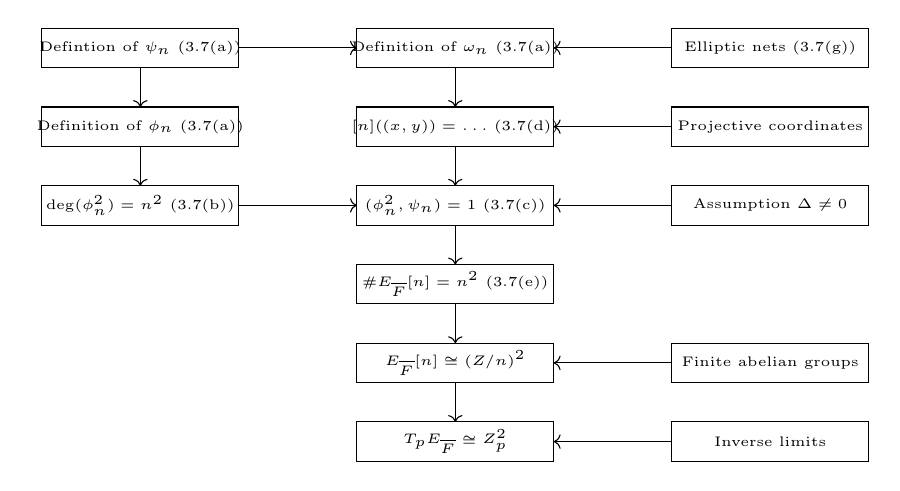
\begin{tikzpicture}
\draw (0, 0) rectangle node{\tiny Defintion of $ \psi_n $ (3.7(a))} (2.5, -0.5);
\draw [->] (2.5, -0.25) -- (4, -0.25);
\draw [->] (1.25, -0.5) -- (1.25, -1);
\draw (0, -1) rectangle node{\tiny Definition of $ \phi_n $ (3.7(a))} (2.5, -1.5);
\draw [->] (1.25, -1.5) -- (1.25, -2);
\draw (0, -2) rectangle node{\tiny $ \deg(\phi_n^2) = n^2 $ (3.7(b))} (2.5, -2.5);
\draw [->] (2.5, -2.25) -- (4, -2.25);
\draw (4, 0) rectangle node{\tiny Definition of $ \omega_n $ (3.7(a))} (6.5, -0.5);
\draw [->] (5.25, -0.5) -- (5.25, -1);
\draw (4, -1) rectangle node{\tiny $ [n]((x, y)) = \dots $ (3.7(d))} (6.5, -1.5);
\draw [->] (5.25, -1.5) -- (5.25, -2);
\draw (4, -2) rectangle node{\tiny $ (\phi_n^2, \psi_n) = 1 $ (3.7(c))} (6.5, -2.5);
\draw [->] (5.25, -2.5) -- (5.25, -3);
\draw (4, -3) rectangle node{\tiny $ \#E_{\overline{F}}[n] = n^2 $ (3.7(e))} (6.5, -3.5);
\draw [->] (5.25, -3.5) -- (5.25, -4);
\draw (4, -4) rectangle node{\tiny $ E_{\overline{F}}[n] \cong (\mathbb{Z} / n)^2 $} (6.5, -4.5);
\draw [->] (5.25, -4.5) -- (5.25, -5);
\draw (4, -5) rectangle node{\tiny $ T_pE_{\overline{F}} \cong \mathbb{Z}_p^2 $} (6.5, -5.5);
\draw (8, 0) rectangle node{\tiny Elliptic nets (3.7(g))} (10.5, -0.5);
\draw [->] (8, -0.25) -- (6.5, -0.25);
\draw (8, -1) rectangle node{\tiny Projective coordinates} (10.5, -1.5);
\draw [->] (8, -1.25) -- (6.5, -1.25);
\draw (8, -2) rectangle node{\tiny Assumption $ \Delta \ne 0 $} (10.5, -2.5);
\draw [->] (8, -2.25) -- (6.5, -2.25);
\draw (8, -4) rectangle node{\tiny Finite abelian groups} (10.5, -4.5);
\draw [->] (8, -4.25) -- (6.5, -4.25);
\draw (8, -5) rectangle node{\tiny Inverse limits} (10.5, -5.5);
\draw [->] (8, -5.25) -- (6.5, -5.25);
\end{tikzpicture}
$$

\end{frame}

\begin{frame}[t]{Future projects}

Projects without algebraic geometry:
\begin{itemize}
\item algorithms that only use the group law
\item finite fields: the Hasse--Weil bound, the Weil conjectures
\item local fields: the reduction homomorphism, Tate's algorithm, the Neron--Ogg--Shafarevich criterion, the Hasse--Weil L-function
\item number fields: Neron-Tate heights, the Mordell--Weil theorem, Tate--Shafarevich groups, the Birch and Swinnerton-Dyer conjecture
\item complete fields: complex uniformisation, p-adic uniformisation
\end{itemize}

Projects with algebraic geometry:
\begin{itemize}
\item elliptic curves over global function fields
\item the projective scheme associated to an elliptic curve
\item integral models and finite flat group schemes
\item divisors on curves and the Riemann--Roch theorem
\item modular curves and Mazur's theorem
\end{itemize}

\end{frame}

\end{document}